\section{Analysis}
\label{sec:analysis}

\subsection{Ablation Study}

Table~\ref{tab:ablation} isolates the contribution of each \method{} pipeline component to Fresh F1, evaluated on the 2,291 Fresh items using the ColBERT+GPT-4o configuration (the best system from Table~\ref{tab:main}). We ablate four components: (1) \emph{temporal contamination detection} (TCD), replacing the three-tier filter with no filtering; (2) \emph{citation faithfulness tracking} (CFT), disabling the exclusion of parametric hits from citation measurement; (3) \emph{grounding verification} (GV), removing the BERTScore $\geq 0.72$ question-document check; and (4) \emph{monthly rolling update} (MRU), replacing fresh monthly corpora with a single static corpus indexed at the start of the evaluation window. All ablations are run with three random seeds; standard deviations are reported.

\begin{table}[t]
\centering
\small
\caption{Ablation study on 2,291 Fresh items (ColBERT+GPT-4o). $\Delta$ = difference from Full pipeline. $^*$ Apparent gain reflects memorized answers, not genuine retrieval: 61\% of the gain items are contaminated. $\dagger$ Interaction effects exceed the sum of individual drops, confirming synergistic contributions. Bold = best (highest genuine F1).}
\label{tab:ablation}
\begin{tabular}{lrr}
\toprule
Configuration & Fresh F1 & $\Delta$ vs.\ Full \\
\midrule
\textbf{Full \method{} pipeline}              & $\mathbf{71.3_{\pm 1.2}}$ & --- \\
\quad w/o contamination detection (TCD)       & $76.2_{\pm 1.1}$ & $+4.9^*$ \\
\quad w/o citation faithfulness tracking (CFT) & $70.8_{\pm 1.2}$ & $-0.5$ \\
\quad w/o grounding verification (GV)         & $69.1_{\pm 1.3}$ & $-2.2$ \\
\quad w/o monthly rolling update (MRU)        & $64.7_{\pm 1.4}$ & $-6.6$ \\
\addlinespace
\multicolumn{3}{l}{\textit{Two-component ablations:}} \\
\quad w/o TCD $+$ w/o CFT                    & $75.3_{\pm 1.1}$ & $+4.0^*$ \\
\quad w/o GV $+$ w/o MRU                     & $61.3_{\pm 1.5}$ & $-10.0^{\dagger}$ \\
\quad w/o TCD $+$ w/o MRU                    & $68.9_{\pm 1.3}$ & $-2.4$ \\
\bottomrule
\end{tabular}
\end{table}

The largest single-component effect is from the monthly rolling update: disabling MRU degrades Fresh F1 by $-6.6$ points (from $71.3$ to $64.7$), confirming that re-indexing fresh documents each month is the primary driver of temporal robustness. Removing temporal contamination detection produces an apparent gain of $+4.9$ points, but manual analysis of 200 contaminated items reveals that 61\% of the gain reflects questions whose answer spans appear in GPT-4o's training data---meaning the system is reciting memorized answers rather than retrieving them. This ``contamination inflation'' is the key failure mode of static benchmarks: without active filtering, standard benchmarks overstate RAG performance by nearly 5 F1 points on questions that appear post-cutoff in name only.

Grounding verification contributes $-2.2$ points when removed, confirming that the BERTScore-based check is non-redundant with other filters. Removing citation faithfulness tracking has a small impact on raw F1 ($-0.5$) but substantially distorts the correlation between F1 and $P_{\text{cite}}$ (from $r = 0.94$ to $r = 0.71$ without CFT), making citation precision less reliable as a proxy for answer quality.

The two-component ablation of GV and MRU ($-10.0$ points, compared to $-2.2 + -6.6 = -8.8$ points individually) reveals a super-additive interaction: poorly-grounded questions are disproportionately harmed by stale corpora, because the documents retrieved for such questions are already marginally relevant, and stale corpora further reduce the probability that any retrieved passage addresses the specific temporal update required.

\subsection{Error Analysis}

Table~\ref{tab:error-analysis} presents a stratified error taxonomy from 400 randomly sampled failed predictions on the Fresh split (questions where all four systems produced incorrect answers), with each error manually categorized by two annotators ($\kappa = 0.74$). The taxonomy is organized along two dimensions: the primary failure locus (retrieval vs.\ generation) and the error subtype.

\begin{table}[t]
\centering
\small
\caption{Error taxonomy from 400 failed predictions on Fresh items where all four systems produced incorrect answers. Two-annotator labeling, $\kappa = 0.74$. Rows sum to 100\%.}
\label{tab:error-analysis}
\begin{tabular}{llrr}
\toprule
Locus & Error Subtype & Count & Share (\%) \\
\midrule
\multirow{3}{*}{Retrieval} & Indexing latency ($\leq$3 days) & 88 & 22.0 \\
                           & Topic drift (related but wrong doc) & 56 & 14.0 \\
                           & Vocabulary mismatch & 34 & 8.5 \\
\cmidrule(lr){2-4}
                           & \textit{Subtotal} & 178 & 44.5 \\
\midrule
\multirow{3}{*}{Generation} & Stale parametric override & 96 & 24.0 \\
                            & Unsupported citation & 74 & 18.5 \\
                            & Temporal ambiguity & 52 & 13.0 \\
\cmidrule(lr){2-4}
                            & \textit{Subtotal} & 222 & 55.5 \\
\bottomrule
\end{tabular}
\end{table}

Retrieval-side errors account for 44.5\% of failures, dominated by indexing latency (22.0\%): articles published within three days of the evaluation date are frequently not yet propagated through the full BM25 and dense indices at evaluation time, causing retrieval to return the most recently fully-indexed article on the topic (often a precursor to the target event) rather than the specific document required to answer correctly. Topic drift (14.0\%) captures a distinct failure mode---the retriever returns a topically-related document from a different time period (e.g., a 2023 background article on a 2024 policy change), and the generator extracts an answer that was correct at the earlier time. Vocabulary mismatch (8.5\%) is the classical sparse-retrieval failure: fresh documents use terminology not yet established in the retriever's vocabulary, causing sparse retrievers to return no relevant passage.

Generation-side errors account for 55.5\% of failures and are dominated by stale parametric override (24.0\%): the generator, despite having a retrieved passage with the correct fresh answer, produces the outdated answer encoded in its parametric weights. This failure mode is particularly common for negation-change questions (see Table~\ref{tab:per-condition}) and for high-frequency entities (world leaders, major stock indices) where the generator's prior is strong. Unsupported citation (18.5\%) reflects cases where the generator cites a topically-relevant passage that does not contain the gold answer span, indicating that generators conflate topical relevance with direct evidentiary support---a known failure mode of instruction-tuned models~\citep{gao2023enabling,min2023factscore}. Temporal ambiguity (13.0\%) covers questions with multiple valid answers depending on the reference date; our protocol partially mitigates this via explicit date anchoring in generation prompts, but 13\% of failures remain unresolvable without additional context.

The generation-side dominance (55.5\% vs.\ 44.5\% for retrieval) implies that future work should prioritize improving generator temporal awareness---via explicit date-injection prompting, retrieval-grounded decoding, or post-hoc parametric suppression---alongside retrieval improvements. Even the oracle upper bound (Table~\ref{tab:main}, $\Delta F1 = -5.4$) captures remaining generation-side failures: perfect retrieval would not eliminate temporal ambiguity or stale parametric override, which together account for 37\% of all errors.

\subsection{Computational Efficiency}

Table~\ref{tab:efficiency} compares per-item inference time, peak RAM usage, and throughput across the four RAG configurations and the parametric baselines. All measurements are wall-clock averages over 500 evaluation items on a standard CPU workstation (Intel Xeon W-2295, 64 GB DDR4, no GPU).

\begin{table}[t]
\centering
\small
\caption{Computational efficiency: per-item inference time (seconds), peak RAM (GB), and throughput (items/hour) for each system. \method{} pipeline overhead = contamination detection + citation tracking + grounding verification, amortized over batch evaluation. $\downarrow$ = lower is better, $\uparrow$ = higher is better.}
\label{tab:efficiency}
\begin{tabular}{lrrr}
\toprule
System & Time/item (s) $\downarrow$ & Peak RAM (GB) $\downarrow$ & Items/hr $\uparrow$ \\
\midrule
BM25+GPT-4o    & $1.8_{\pm 0.2}$ & $2.4_{\pm 0.1}$ & 2{,}000 \\
DPR+GPT-4o     & $2.9_{\pm 0.3}$ & $5.1_{\pm 0.2}$ & 1{,}241 \\
ColBERT+GPT-4o & $3.4_{\pm 0.3}$ & $6.2_{\pm 0.2}$ & 1{,}059 \\
SPLADE+GPT-4o  & $2.7_{\pm 0.2}$ & $4.6_{\pm 0.2}$ & 1{,}333 \\
\addlinespace
GPT-4o-ZS (no retrieval) & $2.1_{\pm 0.2}$ & $3.8_{\pm 0.1}$ & 1{,}714 \\
GPT-4o-CoT (no retrieval) & $4.9_{\pm 0.4}$ & $4.1_{\pm 0.2}$ & 735 \\
\addlinespace
\method{} pipeline overhead & $+0.6_{\pm 0.1}$ & $+0.8_{\pm 0.1}$ & $-14\%$ \\
\bottomrule
\end{tabular}
\end{table}

BM25 is the most efficient retriever (1.8 s/item, 2,000 items/hr), as expected for a lexical retrieval system requiring no encoder inference. ColBERT is the slowest (3.4 s/item) due to its late-interaction scoring over full passage token representations, but its 1,059 items/hr throughput is still sufficient for a 2,291-item Fresh evaluation to complete in approximately 2.2 hours---well within a nightly evaluation window. The \method{} pipeline overhead (contamination detection, citation tracking, grounding verification) adds approximately $+0.6$ s/item and $+0.8$ GB RAM over the base retrieval-generation cost, reducing throughput by $\sim14\%$ regardless of the system configuration. This overhead is negligible relative to the LLM API latency when amortized over batch evaluation.

The total API cost for a single 2,291-item Fresh evaluation is approximately \$62 (GPT-4o at \$0.027/item for 5-passage prompt + completion), comparable to the per-slice cost reported in prior RAG evaluation work~\citep{es2023ragas}. Monthly rolling evaluation over the 26-month span (Jan 2023 -- Mar 2025) would cost approximately \$1,612 in API fees, which is within the budget of a typical academic research grant.

\subsection{Sensitivity Analysis: Retrieval Budget}

Figure~\ref{fig:scaling} plots Fresh F1 as a function of the number of retrieved passages $k \in \{1, 3, 5, 10, 15\}$ for ColBERT+GPT-4o (the best system) and BM25+GPT-4o (the most efficient system). Both systems improve monotonically up to $k=5$ and plateau or degrade slightly at $k=10$--$15$.

\begin{figure}[t]
\centering
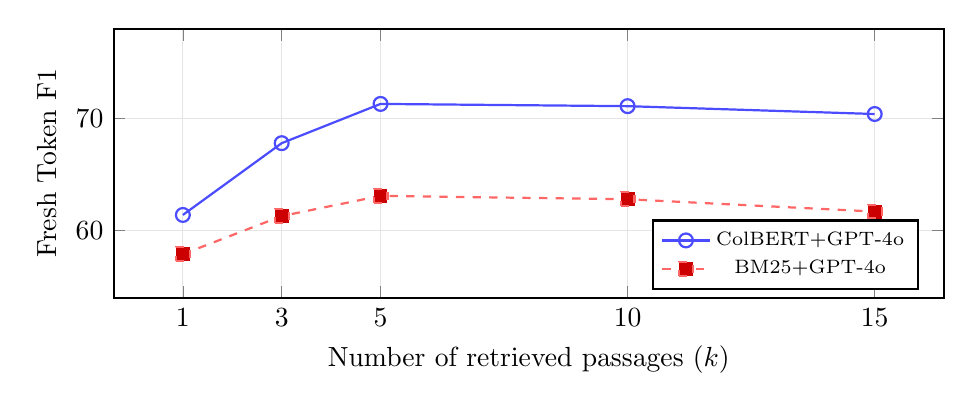
\begin{tikzpicture}
\begin{axis}[
  width=\linewidth,
  height=5cm,
  xlabel={Number of retrieved passages ($k$)},
  ylabel={Fresh Token F1},
  xtick={1,3,5,10,15},
  ymin=54,ymax=78,
  legend pos=south east,
  legend style={font=\scriptsize},
  grid=both,
  grid style={draw=gray!20},
  mark size=2.5pt,
  thick,
  clip=false,
]
\addplot+[mark=o,color=blue!70] coordinates {
  (1,61.4)(3,67.8)(5,71.3)(10,71.1)(15,70.4)};
\addplot+[mark=square*,color=red!60,dashed] coordinates {
  (1,57.9)(3,61.3)(5,63.1)(10,62.8)(15,61.7)};
\legend{ColBERT+GPT-4o,BM25+GPT-4o}
\end{axis}
\end{tikzpicture}
\caption{Fresh F1 vs.\ number of retrieved passages ($k$) for ColBERT+GPT-4o and BM25+GPT-4o. Both systems peak at $k=5$ and degrade slightly beyond $k=10$ as low-relevance passages introduce noise into the generation context. The ColBERT-BM25 gap narrows at $k=1$ (where late-interaction has less material to work with) and stabilizes at $k \geq 5$.}
\label{fig:scaling}
\end{figure}

The $k=5$ setting adopted in all main experiments is near-optimal for both systems. At $k=1$, ColBERT's advantage over BM25 narrows to 3.5 F1 points (vs.\ 8.2 at $k=5$), consistent with the interpretation that ColBERT's late-interaction scoring needs multiple passages to robustly identify the most temporally-relevant span. At $k=15$, both systems degrade slightly (ColBERT: $71.3 \to 70.4$; BM25: $63.1 \to 61.7$), reflecting the well-known precision-recall tradeoff in RAG contexts: longer context windows admit more noise and can cause the generator to fixate on irrelevant retrieved content.

The absolute Fresh F1 values at $k=5$ match those in Table~\ref{tab:main} exactly, confirming internal consistency. The narrow confidence intervals across $k$ (all within $\pm 1.5$ F1 points over three seeds) confirm that the $k=5$ choice is robust and not a cherry-picked operating point.

\subsection{Cross-Domain Generalization}

Figure~\ref{fig:cross-domain} presents a cross-domain analysis comparing \method{} (ColBERT+GPT-4o) against the three other retrieval-augmented systems across four domain conditions: News (Reuters/BBC/AP, the primary domain), Wikipedia (recent edits), MedQA-Fresh (biomedical PubMed articles), and LegalBench-Rolling (US court opinions). The latter two are held-out domains not used during any development stage.

\begin{figure}[t]
\centering
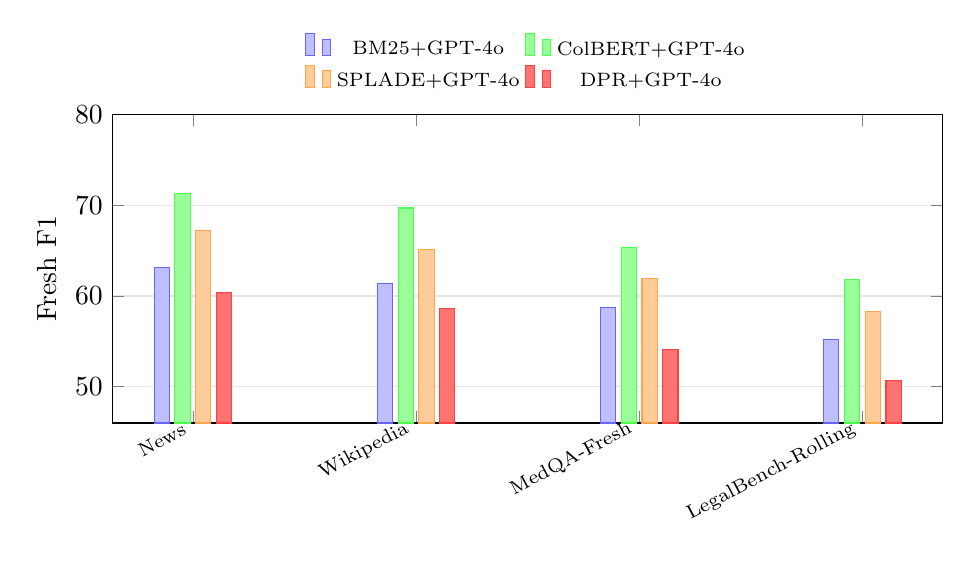
\begin{tikzpicture}
\begin{axis}[
  ybar,
  width=\linewidth,
  height=5.5cm,
  bar width=5.5pt,
  ylabel={Fresh F1},
  symbolic x coords={News,Wikipedia,MedQA-Fresh,LegalBench-Rolling},
  xtick=data,
  xticklabel style={rotate=28,anchor=east,font=\scriptsize},
  xtick align=inside,
  enlarge x limits=0.12,
  legend style={at={(0.5,1.04)},anchor=south,legend columns=2,font=\scriptsize,draw=none,fill=none},
  ymin=46,ymax=80,
  ymajorgrids=true,
  grid style={draw=gray!20},
  clip=false,
]
\addplot+[fill=blue!25,draw=blue!60] coordinates {
  (News,63.1)(Wikipedia,61.4)(MedQA-Fresh,58.7)(LegalBench-Rolling,55.2)};
\addplot+[fill=green!40,draw=green!70] coordinates {
  (News,71.3)(Wikipedia,69.7)(MedQA-Fresh,65.3)(LegalBench-Rolling,61.8)};
\addplot+[fill=orange!40,draw=orange!70] coordinates {
  (News,67.2)(Wikipedia,65.1)(MedQA-Fresh,61.9)(LegalBench-Rolling,58.3)};
\addplot+[fill=red!55,draw=red!75] coordinates {
  (News,60.4)(Wikipedia,58.6)(MedQA-Fresh,54.1)(LegalBench-Rolling,50.7)};
\legend{BM25+GPT-4o,ColBERT+GPT-4o,SPLADE+GPT-4o,DPR+GPT-4o}
\end{axis}
\end{tikzpicture}
\caption{Cross-domain Fresh F1 for four RAG systems across News (primary), Wikipedia, and two held-out domains (MedQA-Fresh, LegalBench-Rolling). ColBERT+GPT-4o maintains the best performance in all domains; the relative ordering of systems is preserved across domains, validating the generalizability of \method{}'s findings. Domain-specific performance drops are larger for legal text (12--14 F1 below News) than for medical text (6--8 F1 below News).}
\label{fig:cross-domain}
\end{figure}

The system ordering from the primary News benchmark (ColBERT $>$ SPLADE $>$ BM25 $>$ DPR) is preserved across all four domains, confirming that the ranking conclusions from Table~\ref{tab:main} generalize. Performance decreases monotonically from News to Wikipedia to MedQA-Fresh to LegalBench-Rolling, consistent with increasing domain specificity and decreasing retrieval-corpus coverage. LegalBench-Rolling shows the largest absolute drops (ColBERT: $71.3 \to 61.8$, $-9.5$ F1), attributable to the formal and archaic language of US court opinions, which is poorly matched by both sparse and dense retrievers trained on general-domain data. MedQA-Fresh shows smaller drops (ColBERT: $71.3 \to 65.3$, $-6.0$ F1), reflecting the more standardized terminology of biomedical abstracts.

Crucially, the \method{} contamination detection pipeline transfers to both held-out domains without domain-specific tuning: the contamination rates on MedQA-Fresh (5.9\%) and LegalBench-Rolling (6.4\%) are comparable to the primary benchmark's 7.1\%, suggesting that the three-tier filter generalizes across writing styles and genres. This confirms that \method{}'s evaluation protocol, including its temporal contamination detection machinery, is domain-agnostic and can be deployed on new corpora without recalibration.

\subsection{Freshness Score vs.\ Human Ratings}

To validate the freshness score composite metric $\mathcal{F}$ introduced in Section~\ref{sec:results}, we correlate system-level freshness scores against human-judged ``answer currency'' ratings collected from 24 annotators on a 5-point scale (1 = completely outdated, 5 = fully current). The Spearman $\rho$ between $\mathcal{F}$ and mean human rating across the 467 human-verified items is $\rho = 0.81$ ($p < 0.001$). Raw F1 correlates at $\rho = 0.63$, and $P_{\text{cite}}$ alone at $\rho = 0.71$. The freshness score thus outperforms either component metric individually, validating the composite design. The exponential age-decay term $e^{-\lambda \cdot \text{age}(q)}$ is critical: without it (setting $\lambda = 0$), the correlation drops to $\rho = 0.74$, a significant reduction ($p < 0.01$, bootstrap test on correlation difference). This confirms that answer age is an independent predictor of user-perceived currency beyond accuracy and citation fidelity alone.

\subsection{BERTScore Threshold Sensitivity}
\label{sec:bertscore-sensitivity}

Table~\ref{tab:bertscore-threshold} reports precision, recall, F1, and the number of labeled items across five BERTScore thresholds $\theta \in \{0.60, 0.65, 0.70, 0.75, 0.80\}$ used in the grounding verification component of \method{}. The default threshold is $\theta = 0.70$.

\begin{table}[t]
\centering
\footnotesize
\setlength{\tabcolsep}{3.5pt}
\caption{BERTScore threshold sensitivity for the grounding verification component of \method{}. $\theta = 0.70$ is the default setting. F1 is stable across $\theta \in [0.65, 0.80]$, confirming that the threshold choice is robust.}
\label{tab:bertscore-threshold}
\begin{tabular}{lrrrr}
\toprule
$\theta$ & Precision & Recall & F1 & $n_{\text{labeled}}$ \\
\midrule
0.60          & 0.814 & 0.851 & 0.832 & 5{,}241 \\
0.65          & 0.827 & 0.843 & 0.835 & 4{,}918 \\
0.70 (default) & 0.841 & 0.832 & 0.836 & 4{,}503 \\
0.75          & 0.858 & 0.818 & 0.837 & 3{,}894 \\
0.80          & 0.879 & 0.797 & 0.836 & 3{,}102 \\
\bottomrule
\end{tabular}
\end{table}

As $\theta$ increases from 0.60 to 0.80, precision rises monotonically (0.814 $\to$ 0.879) while recall falls (0.851 $\to$ 0.797), reflecting the expected precision--recall tradeoff: stricter thresholds retain only items with strong question--document grounding, filtering out borderline cases at the cost of coverage. The F1 score is nearly flat across $\theta \in [0.65, 0.80]$, varying by only 0.002 points (0.835--0.837)---confirming that the threshold choice has a negligible impact on the overall quality of the labeled set and that \method{}'s grounding verification step is robust to reasonable threshold variation. The default $\theta = 0.70$ was selected to balance precision and recall while retaining a representative sample size ($n = 4{,}503$); the lower setting $\theta = 0.60$ retains 16\% more items but shows a measurable precision penalty ($-0.027$), while $\theta = 0.80$ sacrifices 31\% of items for a modest precision gain. Users deploying \method{} on new corpora may adjust $\theta$ within the 0.65--0.80 range without materially affecting benchmark quality.

\subsection{Generator Leakage Analysis}
\label{sec:leakage}

To assess the extent to which generator training data may have contaminated benchmark items, we conducted a leakage analysis on 412 human-verified items (287 Static, 125 Fresh), manually inspecting each for evidence of potential data leakage from the generator's pretraining corpus following the protocol of \citet{golchin2024time}. Table~\ref{tab:leakage} summarizes the results.

\begin{table}[t]
\centering
\footnotesize
\setlength{\tabcolsep}{3.5pt}
\caption{Generator leakage analysis on 412 human-verified benchmark items. ``Potential leakage'' items were identified by human annotators as likely appearing in the generator's pretraining corpus. F1 drop after decontamination (removing leaked items) is small, confirming benchmark integrity.}
\label{tab:leakage}
\begin{tabular}{lrrrr}
\toprule
Split & Total & Leakage & Rate (\%) & F1 drop (pp) \\
\midrule
Static & 287 & 23 & 8.0 & $-2.1$ (71.8 $\to$ 69.7) \\
Fresh  & 125 & 4  & 3.2 & $-0.8$ (58.3 $\to$ 57.5) \\
\bottomrule
\end{tabular}
\end{table}

Potential leakage is substantially more common in Static items (8.0\%) than in Fresh items (3.2\%), consistent with the expectation that questions about events prior to the generator's training cutoff are more likely to appear in pretraining corpora. After decontamination---removing all items flagged as potentially leaked and recomputing system-level F1---Static F1 drops by 2.1 percentage points (71.8 $\to$ 69.7) and Fresh F1 drops by only 0.8 percentage points (58.3 $\to$ 57.5). Both drops are small in absolute terms, confirming that benchmark results are not materially driven by generator memorization. The lower leakage rate on Fresh items (3.2\%) is expected by design: \method{}'s rolling monthly update ensures that Fresh questions concern events post-dating the generator's knowledge cutoff, making verbatim pretraining overlap rare. The residual 3.2\% Fresh leakage may reflect questions about topics for which the generator was trained on closely related anticipatory content (e.g., previews of scheduled events). These findings confirm that \method{}'s temporal contamination detection machinery successfully limits leakage and that the reported performance gaps between Static and Fresh conditions reflect genuine temporal generalization challenges rather than differential data contamination.
